\documentclass{beamer}

\mode<presentation>
{
  \setbeamertemplate{navigation symbols}{}
  \setbeamertemplate{caption}[numbered]
  \setbeamertemplate{footline}[frame number]
} 
% \beamertemplatenavigationsymbolsempty

\usepackage[english]{babel}
\usepackage[utf8]{inputenc}
% \usepackage[numbers]{natbib}
\usepackage{natbib}

% \usepackage{lipsum}

\usepackage{mathtext}
\usepackage[T2A]{fontenc}

\setcounter{tocdepth}{1}

\usepackage{amsmath,amssymb}
\usepackage{tikz}
\usetikzlibrary{matrix,positioning,decorations.pathreplacing}


\usepackage{graphicx}
\usepackage{xcolor}
\usepackage{caption}
\usepackage{grffile}

\graphicspath{{../../assets/}}

\newcommand{\real}{\mathbb{R}}
\newcommand{\cplx}{\mathbb{C}}
\newcommand{\conj}[1]{\overline{#1}}
% \newcommand{\iu}{{\imath}}
\newcommand{\iu}{{\jmath}}
% \newcommand{\iu}{{\mathrm{i}}}
% \newcommand{\iu}{{i\mkern1mu}}

\title[Exam]{Bayesian Sparsification of Deep Complex-valued networks}

\author[Nazarov I., Burnaev E.]{Nazarov Ivan, Burnaev Evgeny}

\date{\today}

\institute[Skoltech]{Skolkovo Institute of Science and Technology}

\begin{document}

\begin{frame}[c,plain,noframenumbering]
  \titlepage
\end{frame}

% \begin{frame}[c]{Summary}
%   \begin{enumerate}
%     \item Complex-valued neural networks (CVNN) offer superior performance in naturally $\cplx$-valued data
%     \medskip
%     \item A CVNN uses half as many floats, but requires double the flops
%     \medskip
%     \item So inducing sparsity becomes important for lower arithmetic complexity
%     \medskip
%     \item To this end we propose $\cplx$ variant of Sparse Variational Dropout
%     \medskip
%     \item Validate the technique by exploring the performance-compression frontier
%   \end{enumerate}
% \end{frame}

\section{$\cplx$-valued neural networks} % (fold)
\label{sec:complex_valued_networks}

\begin{frame}[c]{\insertsection: Motivation}

  Rectangular form: $z = \Re{z} + \iu \Im{z}$, $\iu^2 = -1$
  \begin{itemize}
    \item $\Re{z}$ and $\Im{z}$ are \textbf{real} and \textbf{imaginary} parts of $z$
  \end{itemize}

  Polar form: $z = r e^{\iu \phi}$
  \begin{itemize}
    \item $r = \lvert z \rvert$ -- modulus, $\phi = \arg{\!(z)}$ -- argument of $z$
  \end{itemize}

  \bigskip
  Benefits of using complex numbers $\cplx$ in neural networks
  \begin{itemize}
    \item Richer representation via phase and amplitude $
        r e^{\,\iu \phi} \in \cplx
      $,
      {\tiny \\ \quad
        \citep{reichert_neuronal_2014}}
        \smallskip
    \item Non-degenerate combined phase-amplitude transformations,
      {\tiny \\ \quad
        \citep{hirose_generalization_2012}}
    \smallskip
    % \item ability to compute multiscale windowed spectra
    %   {\tiny \\ \quad
    %     \citep{bruna_mathematical_2015}}
    % \smallskip
    \item Stable BPTT in RNN via unitary transition matrices,
      {\tiny \\ \quad
        \citep{arjovsky_unitary_2016,wisdom_full-capacity_2016}}
  \end{itemize}

\end{frame}

\begin{frame}[c]{\insertsection: Applications}
%  * applications with 
%  * list of references which consider complex-valued networks and their application and motivation
  Natural $\cplx$-valued data representation
  \begin{itemize}
    \smallskip
    \item radar and sattelite imaging
      {\tiny \\ \quad
        \citep{hirose_complex-valued_2009,hansch_complex-valued_2010,zhang_complex-valued_2017}}
    \smallskip
    \item magnetic resonance imaging
      {\tiny \\ \quad
        \citep{hui_mri_1995,wang_deepcomplexmri_2020}}
    \smallskip
    \item radio signal classification
      {\tiny \\ \quad
        \citep{yang_complex_2019,tarver_design_2019}}
    \smallskip
    \item spectral speech modelling and music transcription
      {\tiny \\ \quad
        \citep{wisdom_full-capacity_2016,trabelsi_deep_2018,yang_complex_2019}}
  \end{itemize}
  \medskip
  % key impediment: what 
  % Timeline
  % % $\cplx$-valued convolutional NN 
  % \citep{hansch_complex-valued_2010} later \citep{popa_complex-valued_2017,zhang_complex-valued_2017}
  % % $\cplx$ RNN with holographic associative memory
  % \citep{danihelka_associative_2016}
  % % unitary transition matrices
  % \citep{wisdom_full-capacity_2016}
  % % $\cplx$-valued Batchnorm and Init
  % \citep{trabelsi_deep_2018}
  % % complex-valued transformer
  % \citet{yang_complex_2019}
  % % quaternion netwroks
  % \citep{gaudet_deep_2018}
  Exploring benefits beyond $\cplx$-valued data
  \begin{itemize}
    \item sequence modelling, dynamical system identification
      {\tiny \\ \quad
        \citep{danihelka_associative_2016,wisdom_full-capacity_2016}}
    \smallskip
    \item image classification, road~/~lane segmentation  % KITTI Road Estimation
      {\tiny \\ \quad
        \citep{popa_complex-valued_2017,trabelsi_deep_2018,gaudet_deep_2018}}
  \end{itemize}
\end{frame}

\begin{frame}[c]{\insertsection: Implementation}
  % main reference \citep{trabelsi_deep_2018}, but need some historical perspective
  % $\cplx$VNN operate on complex numbers $\cplx$ instead of real numbers $\real$

  % \medskip
  % \citep{arjovsky_unitary_2016,wisdom_full-capacity_2016,trabelsi_deep_2018,gaudet_deep_2018}
  An intricate double-$\real$ network that respects $\cplx$-arithmetic
  \vspace{-1em}
  \begin{columns}[T]
    \begin{column}{0.45\linewidth}
      \begin{figure}
        % \begin{center}
          % https://tex.stackexchange.com/questions/176432/block-matrix-equation-with-dimensioning

% \documentclass{article}

% \usepackage{tikz}
% \usetikzlibrary{matrix,positioning,decorations.pathreplacing}

% \begin{document}


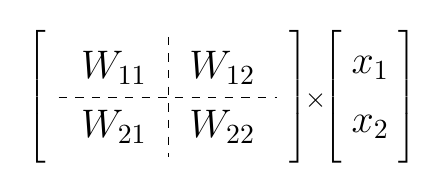
\begin{tikzpicture}[
  style1/.style={
    matrix of math nodes,
    every node/.append style={text width=#1,align=center,minimum height=2.5ex},
    nodes in empty cells,
    left delimiter=[,
    right delimiter=],
    }
  ]
  \matrix[style1=3ex] (1mat)
  {
    & & & \\
    & & & \\
    & & & \\
    & & & \\
  };
  \draw[dashed]
    (1mat-1-2.north east) -- (1mat-4-2.south east);
  \draw[dashed]
    (1mat-2-1.south west) -- (1mat-2-4.south east);
  % \draw[dashed]
  %   (1mat-6-2.south east) -- (1mat-9-2.south east);
  \node[font=\Large]
    at (1mat-1-1.south east) {$W_{11}$};
  \node[font=\Large]
    at (1mat-1-3.south east) {$W_{12}$};
  \node[font=\Large]
    at (1mat-3-1.south east) {$W_{21}$};
  \node[font=\Large]
    at (1mat-3-3.south east) {$W_{22}$};

  \node at ([xshift=2.5ex,yshift=-1.2pt]1mat.east) {$\times$};

  \matrix[style1=1ex,right=5ex of 1mat] (2mat)
  {
    \\
    \\
    \\
    \\
  };
  % \draw[dashed]
  %   (2mat-2-1.south west) -- (2mat-2-1.south east);
  \node[font=\Large] 
    at (2mat-1-1.south) {$x_{1}$};
  \node[font=\Large] 
    at (2mat-3-1.south) {$x_{2}$};
\end{tikzpicture}

% \end{document}

        % \end{center}
        {$\real$VNN linear operation}
        % {$\real$VNN $W x$}
      \end{figure}
    \end{column}%
    \begin{column}{0.45\linewidth}
      \begin{figure}
        % \begin{center}
          % https://tex.stackexchange.com/questions/176432/block-matrix-equation-with-dimensioning

% \documentclass{article}

% \usepackage{tikz}
% \usetikzlibrary{matrix,positioning,decorations.pathreplacing}

% \begin{document}


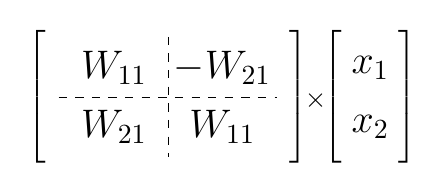
\begin{tikzpicture}[
  style1/.style={
    matrix of math nodes,
    every node/.append style={text width=#1,align=center,minimum height=2.5ex},
    nodes in empty cells,
    left delimiter=[,
    right delimiter=],
    }
  ]
  \matrix[style1=3ex] (1mat)
  {
    & & & \\
    & & & \\
    & & & \\
    & & & \\
  };
  \draw[dashed]
    (1mat-1-2.north east) -- (1mat-4-2.south east);
  \draw[dashed]
    (1mat-2-1.south west) -- (1mat-2-4.south east);
  % \draw[dashed]
  %   (1mat-6-2.south east) -- (1mat-9-2.south east);
  \node[font=\Large]
    at (1mat-1-1.south east) {$W_{11}$};
  \node[font=\Large]
    at (1mat-1-3.south east) {$-W_{21}$};
  \node[font=\Large]
    at (1mat-3-1.south east) {$ W_{21}$};
  \node[font=\Large]
    at (1mat-3-3.south east) {$W_{11}$};

  \node at ([xshift=2.5ex,yshift=-1.2pt]1mat.east) {$\times$};

  \matrix[style1=1ex,right=5ex of 1mat] (2mat)
  {
    \\
    \\
    \\
    \\
  };
  % \draw[dashed]
  %   (2mat-2-1.south west) -- (2mat-2-1.south east);
  \node[font=\Large] 
    at (2mat-1-1.south) {$x_1$};
  \node[font=\Large] 
    at (2mat-3-1.south) {$x_2$};
\end{tikzpicture}

% \end{document}

        % \end{center}
        {$\cplx$VNN linear operation}
        % {$\cplx$VNN $(W_{11} + iW_{21}) (x_1 + i x_2)$ }
      \end{figure}
    \end{column}
  \end{columns}

  \bigskip
  % \item nonlinearities: trigonometric, real-imaginary ReLU etc.
  Activations
  \begin{itemize}
    \item split $
      z \mapsto g(\Re{z}) + \iu g(\Im{z}) % split
    $ or $
      z \mapsto g(\lvert z\rvert) e^{\iu \arg{\!(z)}}
    $ % \citep{trabelsi_deep_2018,hirose_generalization_2012,reichert_neuronal_2014} % relu, tanh, sigmoid
    \item full: trigonometric, holomorphic
  \end{itemize}
  % \citep{hirose_complex-valued_2009}  argues that holomorphy and nondifferentiability are non-issues

  \smallskip
  Geometric representation $\cplx \simeq \real^2$ for backpropagation
  % REWRITE THIS
  \begin{itemize}
    \item Wirtinger calculus: independent $z$ and ${\conj{z}}$ $
        \partial_z
      $ and $
        \partial_{\conj{z}}
      $
    \item $\nabla_z L = \partial_{\conj{z}} L(z)$ for $L\colon \cplx^m \to \real$
    % \citep{zimmermann_comparison_2011}
  \end{itemize}
    % \cite{trabelsi_deep_2018}, \cite{arjovsky_unitary_2016}
  % So essentially implementing $\cplx$-valued networks boils down consistently
  % structured $\real$-valued with double the dimensions.
\end{frame}

% section complex_valued_networks (end)

\section{Sparsity and compression} % (fold)
\label{sec:compression}

\begin{frame}[c]{\insertsection}
% Compression is not just making the nets smaller, it is also
% making them use less artihmetic operations, or faster ops
  Improve power, storage or throughput efficiency of deep nets:
  \begin{itemize}
    \item Knowledge distillation
      {\tiny \\ \quad
        \citep{hinton_distilling_2015,balasubramanian_deep_2016}}
    \item Network pruning
      {\tiny \\ \quad
        \citep{lecun_optimal_1990,seide_conversational_2011,zhu_prune_2018}}
    \item Low-rank matrix~/~tensor decomposition
      {\tiny \\ \quad
        \citep{denton_exploiting_2014,novikov_tensorizing_2015}}
    \item Quantization and fixed point arithmetic
      {\tiny \\ \quad
        \citep{courbariaux_training_2015,han_deep_2016,chen_fxpnet_2017}}
  \end{itemize}
% Making them smaller or using faster ops:
% * Knowledge distillation -- creating a smaller replica
% * low-rank approximations -- low-rank structure with efficient mat-vec operations
% * quantization -- dynamic range of floating-points to fixed-points and use fixed range int arithmetic
% * sparsisty -- inducing regularizers (lasso)
% * pruning -- remove insignificant parameters

  \bigskip
  Applications to $\cplx$VNN:
  \begin{itemize}
    \item $\cplx$ modulus pruning, quantization with $k$-means in $
        \real^2%\simeq \cplx
      $, 
      {\tiny \\ \quad
        \citep{wu_compressing_2019}}
    \item $\ell_1$ regularization for hyper-complex-valued networks,
      {\tiny \\ \quad
        \citep{vecchi_compressing_2020}}
      % same calculus relaxation as in $\cplx\real$ calculus
  \end{itemize}

\end{frame}

\subsection{Sparse Variational Dropout \citep{molchanov_variational_2017}} % (fold)
\label{sub:sparse_variational_dropout}

\begin{frame}[c]{\insertsubsection}{\insertsection}
% started as model regularization method Kingma et al. (2015)
  Variational Inference with automatic relevance determination effect

% decided to go with this term
% Bayesian inference objective: combine prior assumptions with data into posterior beliefs
% VI -> SGVB: Jordan (VI), Hoffman (SVI), Kingma (SGVB) (give the elbo equation)

% Bayesian perspective on dropout proposed by Kingma at al. (2015)
% repurposed for sparsification by Molchanov et al. (2017) and Kharitonov et al. (2018)
  $$
    \underset{
      {\color{orange} q} \in \mathcal{Q}
      % , {\color{teal} \theta}
    }{\text{maximize}}
    \quad
    \underbrace{
      \mathbb{E}_{w \sim {\color{orange} q}}
        % \overbrace{
          \log p(D\mid w)  % ; {\color{teal} \theta})
        % }^{
          % \text{model}
          % \,
          % x\mapsto \hat{y}_w(x)
        % }
    }_{
      \text{data model likelihood}
    }
    \quad
    - \underbrace{
      KL({\color{orange} q}\|{\color{blue} \pi})
    }_{
      \text{variational regularization}
    }
    $$

  % Combine prior assumptions with data into posterior beliefs
  \medskip
  prior ${\color{blue} \pi}$
    $\to$ data model likelihood
    $\to$ posterior ${\color{orange} q}$
    (close to $p(w \mid D)$)
  
  \bigskip
  % Bayesian interpretation of Dropout of \citep{kingma_variational_2015}
  % repurposed for parameter pruning by 
  Factorized Gaussian dropout posterior family $\mathcal{Q}$
  \begin{itemize}
    \item $
      w_{ij} \sim {\color{orange} q}(w_{ij})
        = \mathcal{N}(
          w_{ij}\,\big\vert\,
          {\color{teal} \mu_{ij}},
          {\color{red} \alpha_{ij}}
            {\color{teal} \mu_{ij}}^2
        )
    $, $\alpha_{ij} > 0$, and ${\color{teal} \mu_{ij}} \in \real$
    \item parameter relevance $\propto \frac1{{\color{red} \alpha_{ij}}}$
  \end{itemize}

  \smallskip
  Factorized prior $
    {\color{blue} \pi}(w_{ij})
      \propto \frac1{\lvert w_{ij}\rvert}
  $ (VD)
  \begin{itemize}
    \item (ARD) $
      {\color{blue} \pi}(w_{ij}) = \mathcal{N}(
        w_{ij}\,\big\vert\,
        0, \tfrac1{{\color{teal} \tau_{ij}}}
      )
    $, \citep{kharitonov_variational_2018}
  \end{itemize}
  % precision $\tau_{ij} > 0$
\end{frame}

% subsection sparse_variational_dropout (end)

% section compression (end)

\section{Extension to complex parameters} % (fold)
\label{sec:extension_to_complex_parameters}

\begin{frame}[c]{\insertsection}
% Thechnical contrib
The same objective, but with proper Complex-valued distributions
\begin{itemize}
  \item $
    {\color{orange} q}(w_{ij})
  $ is $\cplx$ Gaussian distribution $
    \mathcal{N}^{\cplx}(
      w_{ij}\,\big\vert\,
      {\color{teal} \mu_{ij}},
      \sigma^2_{ij},
      \gamma_{ij}
    )
  $ with $
    {\color{teal} \mu_{ij}}, \gamma_{ij} \in \cplx
  $, $
    \sigma^2_{ij}
      = {\color{red} \alpha_{ij}}
        \lvert {\color{teal} \mu_{ij}} \rvert^2
  $ such that $\lvert \gamma_{ij}\rvert \leq \sigma^2_{ij}$
  \item put $\gamma_{ij} = 0$: 
    \textbf{real} and \textbf{imaginary} components are independent
\end{itemize} 

Discussion?

\medskip
Complex analogues of the priors
\begin{columns}[T]
  \begin{column}{0.63\linewidth}
    \begin{itemize}
      \item ($\cplx$-VD) $
        {\color{blue} \pi}(w_{ij})
            \propto \lvert w_{ij}\rvert^{-\beta}
      $, $\beta \geq 1$
      \smallskip
      \item ($\cplx$-ARD) $
        {\color{blue} \pi}(w_{ij})
            = \mathcal{N}^{\cplx}(
              w_{ij}\,\big\vert\,
              0, \tfrac1{{\color{teal} \tau_{ij}}}, 0
            )
      $
    \end{itemize}
  \end{column}
  \begin{column}{0.35\linewidth}
    \includegraphics[draft,scale=0.25]{figure/complex-gaussian.png}
    {
      $\mathbb{C}\mathcal{N}(0, 1, \eta e^{\jmath \phi})$
    }
  \end{column}
\end{columns}

\end{frame}

% subsection _cplx_valued_gaussian_distribution (end)

% section extension_to_complex_parameters (end)

\section{Experiments} % (fold)
\label{sec:experiments}

\begin{frame}[c]{\insertsection}
  % methodological contrib
  Variational objective similar to $\beta$-VAE, \citep{higgins_beta-vae_2017}
  \begin{equation}
  \label{eq:beta_elbo}
    \max_q
    \mathbb{E}_{w \sim {\color{orange} q}}
      \log p(y\mid w, x)  % ; {\color{teal} \theta})
    - \beta KL({\color{orange} q}\|{\color{blue} \pi})
    \tag{$\beta$-ELBO}
  \end{equation}
  \begin{itemize}
    \item VAE: control the capacity and statistical independence of the latent
    information through a constraint on the divergence
    \item Variational Dropout: balance the gradient feedback of the loss and the
    prior-matching terms of ELBO (information budgeting, see \citep{BitsBack})
    \item KL-div annealing of \citet{molchanov_variational_2017} does not allow
    to explore the performance-compression trade-off
  \end{itemize}
\end{frame}

\begin{frame}[c]{\insertsection}
  % methodological contrib
  Three-stage training:
  \begin{enumerate}
    \item `pre-train' the network as-is with deterministic layers
    \item `compress' with Variational Dropout layers and \eqref{eq:beta_elbo}
    \item `fine-tune' only relevant parameters using deterministic maskable layers
    % sparse layers are sloooow
  \end{enumerate}

  \medskip
  $w_{ij}$ is relevant, i.e. $m_{ij} = 1$, iff $
    \log{{\color{red} \alpha_{ij}}} \leq \tau
  $ for $\tau = -\tfrac12$
  \begin{itemize}
    \item \citet{molchanov_variational_2017,kingma_variational_2015} use $\tau=3$,
      tied to Bernoulli Dropout with rate $95\%$
    \item We argue, that $q$ is factorized Gaussian, $
        \tfrac{k \lvert w - \mu \rvert^2}
              {\alpha \lvert \mu \rvert^2}
      $ is $\chi^2_k$ distributed with $k=1$ ($\real$) or $2$ ($\cplx$)
    \item relevant parameters are sufficiently concentrated around their mode according
    to the posterior
  \end{itemize}

  A picture of the typical $\log \alpha$ distribution?
\end{frame}

% section experiments (end)

\begin{frame}[t]{\insertsection}
  Image classification
  \begin{itemize}
    \item MNIST, Fashion-MNIST, Kanji-MNIST, EMNIST-Letters
  \end{itemize}
\end{frame}

\section{Results on MusicNet} % (fold)
\label{sec:results_on_musicnet}

\begin{frame}[c]{\insertsection}

Music annotation task on MusicNet \citet{thickstun_learning_2017}
\begin{itemize}
  \item an audio dataset of $330$ annotated musical compositions
  \item use power spectrum to tell which piano keys are pressed
  \item $\cplx$-networks achieve better performance than $\real$-nets,
  \cite{trabelsi_deep_2018}
\end{itemize}
\begin{figure}[t]
  \centering
  \includegraphics[draft,scale=0.25]{figure/stft.png}
  \par
  \includegraphics[draft,scale=0.19]{figure/predicted.png}
\end{figure}

\medskip
current SOTA on MusicNet Average Precision
$\cplx$: 72.9\% \citet{trabelsi_deep_2018} VGG-like $\cplx$-net
$\cplx$: 74.2\% \citet{yang_complex_2019} $\cplx$-transformer
$\real$: 77.3\% \citet{thickstun_invariances_2018} $\real$-network with special
STFT features \citet{citation_needed}

\end{frame}

\begin{frame}[c]{\insertsection}
% We successfully compressed the network for MusicNet from \cite{trabelsi_deep_2018}
Performance-compression trade-off for the $\cplx$-network from \cite{trabelsi_deep_2018}
  \begin{figure}[t]
    \centering
    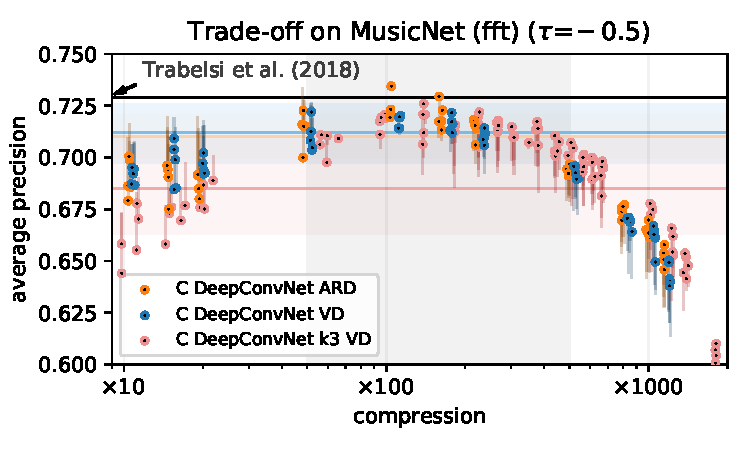
\includegraphics[scale=0.55]{figure__musicnet__trade-off/paper__musicnetram__fft__-0.5.pdf}
  \end{figure}

\end{frame}

\begin{frame}[c]{\insertsection}
  Effects of threshold selection
\end{frame}

% section results_on_musicnet (end)

\section{General Results} % (fold)
\label{sec:general_results}

\begin{frame}[c]{\insertsection}
Experiments on image classification and music transcription
\begin{itemize}
  \item $\cplx$-VD and $\cplx$-ARD equally successfully compress $\cplx$-networks
  \smallskip
  \item Variational Dropout controllably removes redundancy in wide $\cplx$ and $\real$ networks
  \smallskip
  \item $\real$-networks tend to compress better than $\cplx$-nets
\end{itemize}

\bigskip
Compression results are replicable and stable across randomizations
\begin{itemize}
  \item Fine-tuning sparse parameters generally improves performance
\end{itemize}
\end{frame}

% section general_results (end)

\section{Conclusions and Further Developments} % (fold)
\label{sec:conclusions_and_further_developments}

\begin{frame}[c]{\insertsection}
  \begin{columns}[T]
    \begin{column}{0.38\textwidth}
      \begin{itemize}
        \item Extended Bayesian Sparsification method to $\cplx$-valued networks
        \item Empirically explored the compression-performance frontier
      \end{itemize}
    \end{column}
    \begin{column}{0.58\textwidth}
      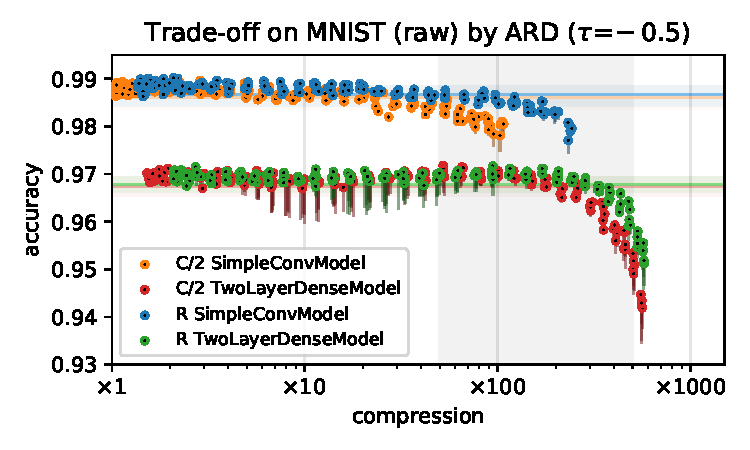
\includegraphics[scale=0.35,clip]{figure__mnist-like__trade-off/appendix__cmp__ARD__mnist__raw__-0.5.pdf}
    \end{column}
  \end{columns}

  \bigskip
  Key limitation: parameter independence % in ${\color{orange} q}$ does not hold in practice
  \begin{itemize}
    \item utilizing parameter coupling may give higher compression
    \item structured sparsity is desirable for SIMD-processing in embedded ML
  \end{itemize}

\end{frame}

% section conclusions_and_further_developments (end)

\section{References} % (fold)
\label{sec:references}

\begin{frame}<beamer:0>[t,noframenumbering,plain,allowframebreaks]{\insertsection}
  \tiny
  \bibliographystyle{abbrvnat}
  \bibliography{presentation}
\end{frame}

% section references (end)

\end{document}
